\begin{figure*}[hbtp]
  \centering
  \subfigure{
    \label{fig:de-lorenz-web-Stanford}
    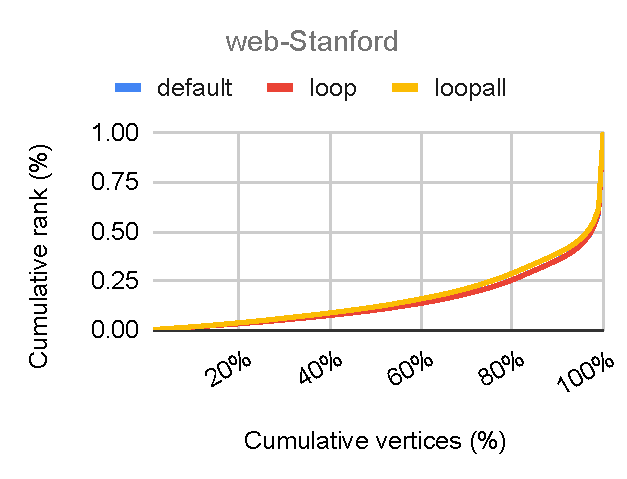
\includegraphics[width=0.31\linewidth]{out/de-lorenz-web-Stanford.pdf}
  }
  \subfigure{
    \label{fig:de-lorenz-arabic-2005}
    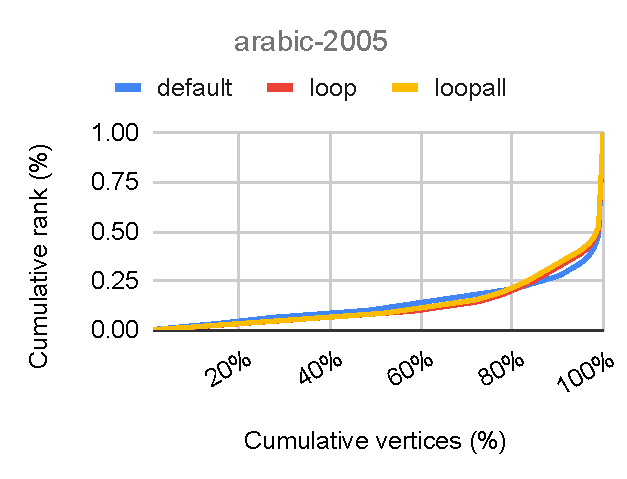
\includegraphics[width=0.31\linewidth]{out/de-lorenz-arabic-2005.pdf}
  }
  \subfigure{
    \label{fig:de-lorenz-soc-Epinions1}
    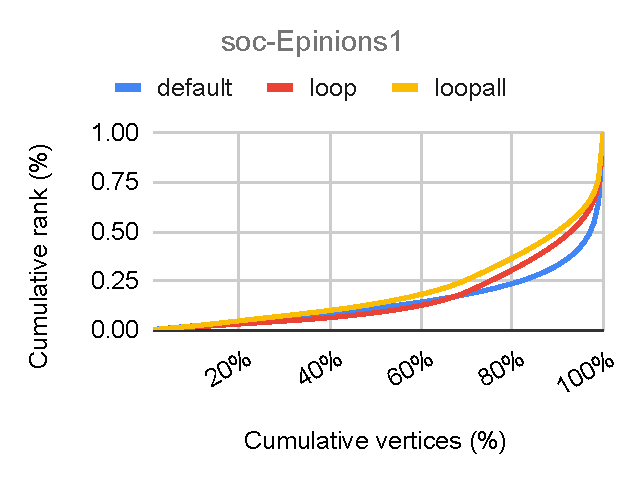
\includegraphics[width=0.31\linewidth]{out/de-lorenz-soc-Epinions1.pdf}
  }
  \subfigure{
    \label{fig:de-lorenz-wiki-Talk}
    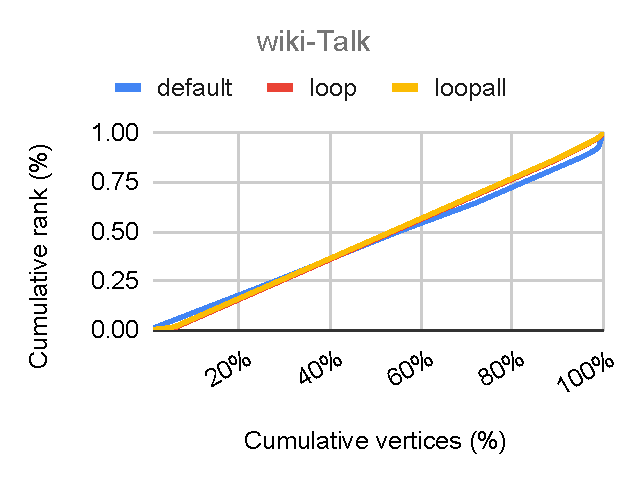
\includegraphics[width=0.31\linewidth]{out/de-lorenz-wiki-Talk.pdf}
  }
  \subfigure{
    \label{fig:de-lorenz-germany_osm}
    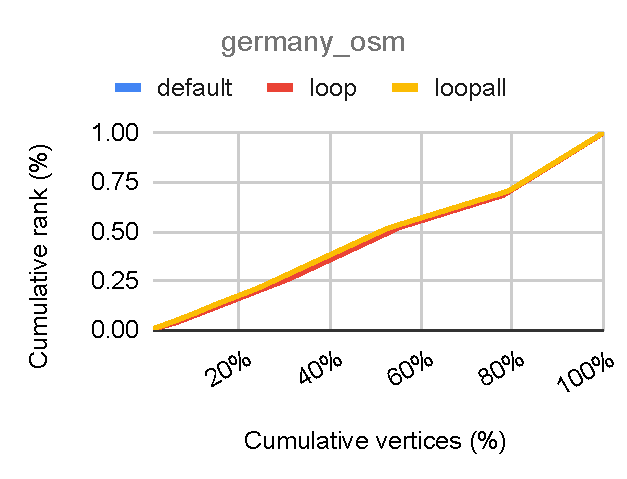
\includegraphics[width=0.31\linewidth]{out/de-lorenz-germany_osm.pdf}
  } \\[-2ex]
  \caption{Lorenz curve of PageRank values on five relevant graphs, comparing between PageRank values obtained with three different dead-end handling strategies: \textit{teleport from dead-ends} (\textbf{default}), \textit{self-loop dead-ends} (\textbf{loop}), and \textit{self-loop all vertices} (\textbf{loopall}). Note that web graphs have high inequality, while communication graphs and road networks little to no inequality.}
  \label{fig:de-lorenz-all}
\end{figure*}
